\documentclass[a4paper, 11pt]{article}
\usepackage{comment} % enables the use of multi-line comments (\ifx \fi) 
\usepackage{lipsum} %This package just generates Lorem Ipsum filler text. 
\usepackage{fullpage} % changes the margin
\usepackage{graphicx}
\usepackage{subfig}
\graphicspath{ {report/} }

\begin{document}
\noindent
\large\textbf{EIASR report} \hfill \textbf{Szymon Michalski} \\
\normalsize 17Z \hfill Fruits and Vegetables Classifier\\


\section*{Task Description}
The project is to create classifier for fruits and vegetables. 
There is given subset of fruits and vegetables: orange, apple, watermelon, cauliflower, broccoli. Additionally there is one more class describing not known objects.
Classifier will give an answer of the type of the object on the input and will also be able to tell if it is an object not from the given list of learned objects.

\section*{Proposed solution}
In order to solve the given problem the following solution was proposed:
Features will be extracted from images via SIFT algorithm. Later features will be added to Bag of Words. Finally images will be classified using Support Vector Machine.

\section*{Scale-Invariant Feature Transform (SIFT)}
SIFT converts each patch to 128-dimensional vector. After this step, each image is a collection of vectors of the same dimension (128 for SIFT).

SIFT consists of few steps:

\begin{enumerate}

\item Difference of Gaussian

Difference of Gaussian is obtained as the difference of Gaussian blurring of an image. This process is done for different octaves of the image in Gaussian Pyramid. Octave is the scale of a feature.

\begin{figure}[!htbp]
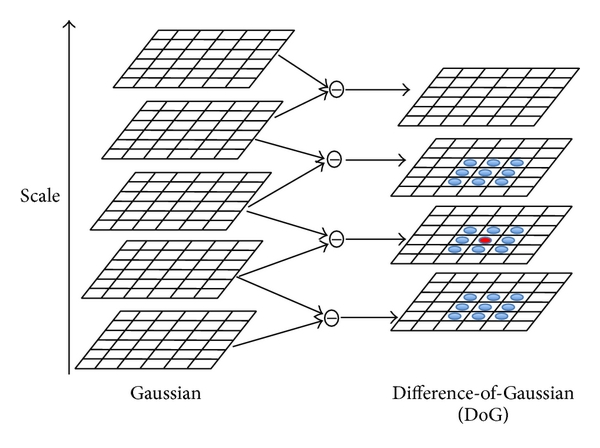
\includegraphics[scale=2.2]{The-process-of-local-extrema-detection-based-on-Difference-of-Gaussian-DoG.png}
\centering
\caption{Difference of Gaussian}
\end{figure}


\item Keypoint detection

Once it is found, images are searched for local extrema over scale and space. If it is a local extrema, it is a potential keypoint. Low-contrast keypoints are filtered out. It means that keypoint is best represented in that scale. For each interesting point its octave, x, and y coordinates are saved as a keypoint. 

\item Orientation assignment

To each keypoint orientation is assigned in order to achieve invariance to image rotation. SIFT features are assigned an orientation based on the pixel intensities of the surrounding area. Gradient magnitude and direction is calculated in that area. An orientation histogram with 36 bins covering 360 degrees is created. The highest peak in the histogram is taken. In simple words each image is turned in such way that the brightest point is in the upper part of image.

\item Keypoint descriptor generation

Finally all keypoints are found: x, y, and octave locations for all points of interest, plus orientation. The keypoints are scale-invariant and rotation-invariant. At the end the output is 128 dimensional vector for each keypoint. The next process is called Histogram of Oriented Gradients (HOG). Gradient in this case describes how pixel's intensity changes between one pixel and another. At this point each keypoint's pixel is converted into gradient, which are later used to build histograms.

\end{enumerate}

\begin{figure}[!htbp]
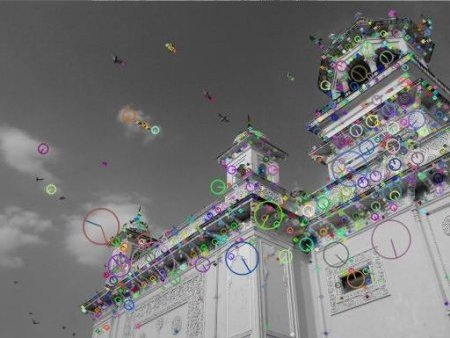
\includegraphics[scale=0.7]{sift_keypoints.jpg}
\centering
\caption{SIFT keypoints}
\end{figure}


\begin{figure}[!htbp]
  \centering
  \subfloat[SIFT keypoint to gradient]{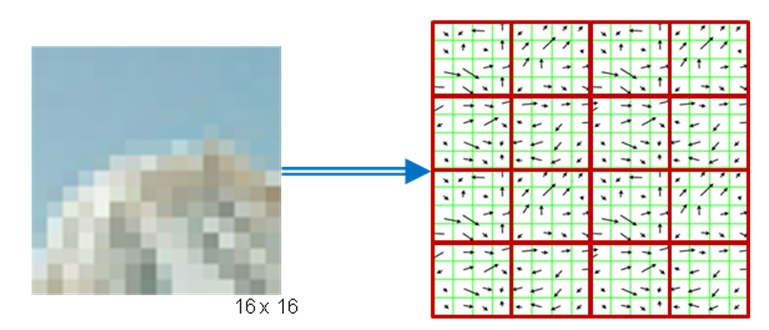
\includegraphics[width=0.8\textwidth]{figure4.jpg}}
  \hfill
  \subfloat[SIFT gradient to histogram]{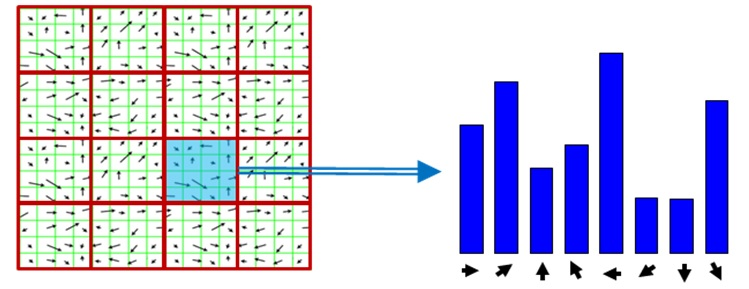
\includegraphics[width=0.8\textwidth]{figure5.jpg}}
  \hfill
  \subfloat[SIFT output histogram]{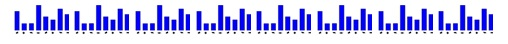
\includegraphics[width=0.8\textwidth]{figure6.jpg}}
  \caption{Example of SIFT gradient.}
\end{figure}


\section*{Bag of Words (BoW)}
When features are found it is possible to group them together. BoW can be understood as "histogram representation based on independent features". 

BoW model has to convert vector-represented patches to "codewords", which creates a "codebook" or "dictionary". A codeword can be considered as a representative of several similar patches. In OpenCV it is used by performing k-means clustering over all vectors. The number of the clusters is the codebook size.

\begin{figure}[!htbp]
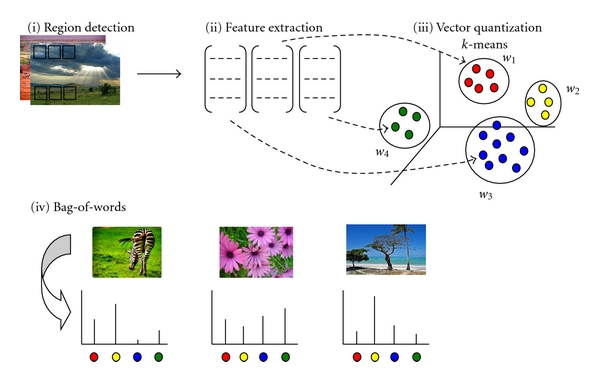
\includegraphics[scale=3]{bow.jpg}
\centering
\caption{BoW example}
\end{figure}


\section*{Support Vector Machine (SVM)}

SVM a supervised machine learning algorithm that is commonly used in classification problems. SVM's basic idea is to find a hyperplane that best divides a dataset into two classes.

Support vectors are the data points nearest to the hyperplane. Those points would alter the position of the dividing hyperplane if would be removed hence are critical elements.

\begin{figure}[!htbp]
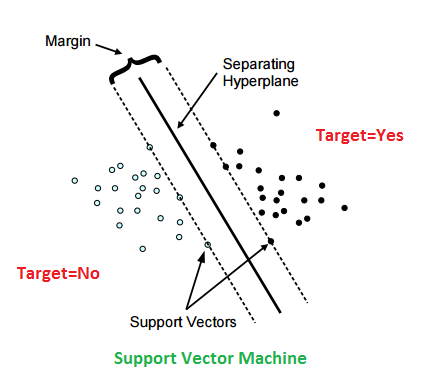
\includegraphics[scale=0.8]{SVM-Planes.png}
\centering
\caption{SVM simple example}
\end{figure}


In case when there is no clean and easy hyperplane to be found (i.e. straight line in 2D plane), then input space has to be transformed into feature space. In case of 2D plane it would be transformed to 3D plane. It is shown in the below image.

\begin{figure}[!htbp]
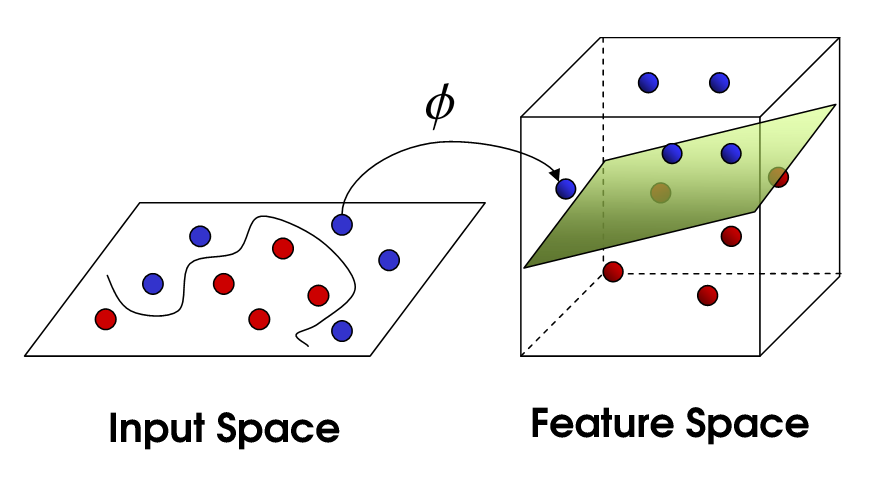
\includegraphics[scale=0.3]{svm.png}
\centering
\caption{SVM transition to feature space example}
\end{figure}


\section*{Testing Images Selection}
Due to lack of prepared dataset of already tagged fruits and vegetables imaged, images were gathered from www.image-net.org and thoroughly checked. Then they were divided into six classes: orange, apple, watermelon, cauliflower, broccoli, other.

\section*{Analysis \& Testing}
Testing can be used for example using 10-fold cross-validation. Analysis can be done basing on the resulting Confusion Matrix.

\end{document}
